%!TEX root = project.tex

\chapter*{About this project}
\paragraph{Abstract}

This project will help to explain the temporal difference reinforcement learning process by displaying an agents behaviour, performance and Q-Table as it interacts within its environment. The application is a browser based visual tool where a user can interact by tweaking parameters within a form. Once the form is submitted it will then make a request to run a main python script held on a flask server. Once the script has completed the user will be presented with and animation of the agent moving through it's environment. In addition a graph of the agent performance and the q-table will presented to the user for examination. This will aid the user in better understanding the concept of reinforcement learning.

\paragraph{Authors}
Kevin Gleeson 4th year student studying Software Development at GMIT Galway.



\chapter{Introduction}
\textbf{Reinforcement learning}\\
\begin{figure}[H]
	\centering
	\includegraphics[width=0.7\linewidth]{"../../../Project Plan/grid_world_env"}
	\caption{}
	\label{fig:gridworldenv}
\end{figure}

Reinforcement learning is the process of rewarding an agent for a decision made within its environment. The reward can be either positive or negative based on the decisions made by the agent as it transitions from one state to another.\\
For example, if a puppy has no knowledge of the sit command it will not perform the desired action on the first attempt. Each time the puppy sits when commanded its decision is reinforced with a positive treat/reward. If the puppy does not sit the reward is negative (no treat). Eventually after many iterations of training, the dog will associate a treat/reward with that specific command and eventually learn that sitting will get them a treat. 
The puppy in essence is taking actions to maximise rewards while exploring an unknown environment.\\
With reinforcement machine learning, this technique is used to train an agent to learn about its environment through trial and error.
The environment used for this project will be grid world. The  grid world domain is a two dimensional grid with the agent starting at the bottom left of the grid, the goal state is at the top right of the grid in addition there are traps that the agent needs to avoid while travelling from the start state to it's goal state.
Reinforcement Learning is an unsupervised machine-learning technique that allows an agent to explore and learn from its environment without any prior knowledge of the domain. With Reinforcement Learning there are the following main components.

Agent:
The agent is an object within the environment that makes decisions based on it's current state space and possible rewards gained by choosing an action. For this application the agent is placed in a two dimensional environment. The possible actions that can be taken by the agent are up, down, left or right.

The environment:
For the purpose of this application a  6 * 6 two dimensional grid environment will be used. As the script is running the agent will move from one square in the grid to the next adjacent square of up, below, to the left or the right of its current position.

As the agent moves through the environment it gains knowledge via reward signals gathered by transitioning from one state to another based on the action taken from its current state.
With each step the agent is only concerned with its current state and what rewards it can gain from transitioning to it's next state.~\cite{}
The agent chooses it's action decision based on what highest reward it can get from the next available states.\\
The purpose of this application is to demonstrate and explain reinforcement learning through a browser based visualisation tool.\\
The application will have the following elements on the Browser:
\begin{itemize}
\item The agent moving within its environment when the simulation is run.\\This will be displayed using HTML 5 canvas.

\item User input to tweak parameters before each run of the simulation. The parameters that will be available to the user are:
	\begin{itemize}
		\item The end goal reward
		\item The negative trap reward
		\item The agent learning rate
		\item The learning decay rate
		\item The discount factor
		\item The Exploration rate
		\item The Exploration decay rate
		\item The per step reward
		\item The maximum number of episodes to be run
		\item The maximum number of agent steps per episode
		\item Choice of algorithm
	\end{itemize}
\end{itemize}







\begin{itemize}
	\item The agent’s actions effect the environment by moving around and exploring.
	\item	The state is what the agent can observe at a given time. In the grid above, the agent can occupy eleven possible squares. We can number theses states from 1 – 11 moving from left to right with the bottom left square being state number 1.
	\item	In the agents initial state (State 1) it knows nothing about its environment and chooses an action of moving left, right, up or down.
	\item	The Epsilon variable sets the probability of choosing a random action. When set to one it will always choose a random action. If set to .8 it will choose the a random action 80\% of the time.
\end{itemize}
This will give the agent a chance to explore the environment depending on what the value is set to.
\begin{itemize}
\item Q values are a weighted score attached to an action of a particular state.
\item There is a negative reward cost for each move the agent makes in this case -0.04. This will help in getting the best path to the end state.
\item The learning rate (alpha) is a value between zero and one determines how much the Q value is updated for each action taken. It will be .5 for this example.
\item The discount factor (Gamma) set to .9 is the immediate reward gained for an action taken. The higher the value the more the agent will take the immediate reward.
\item The reward cost, gamma and alpha are hyper-parameters chosen by the user.
\item There is a formula to follow to update the Q values of each action taken:
Q (current state, action) += alpha *[reward + gamma* max value of Q (next state, all possible actions) – Q (current state, action)]
\item The Q table is a record of all of the agent’s actions taken in a given state. This is the agent’s memory and is set to zero when first run. If all Q values are equal, it will 
Choose one at random.
\end{itemize}




	\begin{tabular}{lllll}
		State & Action left & Action right & Action up & Action down \\
		1     & 0           & 0            & 0         & 0           \\
		2     & 0           & 0            & 0         & 0           \\
		3     & 0           & 0            & 0         & 0           \\
		4     & 0           & 0            & 0         & 0           \\
		5     & 0           & 0            & 0         & 0           \\
		6     & 0           & 0            & 0         & 0           \\
		7     & 0           & 0            & 0         & 0           \\
		8     & 0           & 0            & 0         & 0           \\
		9     & 0           & 0            & 0         & 0           \\
		10    & 0           & 0            & 0         & 0           \\
		11    & 0           & 0            & 0         & 0          
	\end{tabular}
\\
\\
If the agent decides to move up one square to state 5 the Q table is updated using the formula above which looks like   .5 * -.04  + .9 *0 – 0 = -0.02

	\begin{tabular}{lllll}
		State & Action left & Action right & Action up & Action down \\
		1     & 0           & 0            & -0.02     & 0           \\
		2     & 0           & 0            & 0         & 0           \\
		3     & 0           & 0            & 0         & 0           \\
		4     & 0           & 0            & 0         & 0           \\
		5     & 0           & 0            & 0         & 0           \\
		6     & 0           & 0            & 0         & 0           \\
		7     & 0           & 0            & 0         & 0           \\
		8     & 0           & 0            & 0         & 0           \\
		9     & 0           & 0            & 0         & 0           \\
		10    & 0           & 0            & 0         & 0           \\
		11    & 0           & 0            & 0         & 0          
	\end{tabular}
\\
\\
\\
If the Agent decides to move down to state one again the value of moving down from state 5 to state 1 is updated to -0.02 also.
\\

	\begin{tabular}{lllll}
		State & Action left & Action right & Action up & Action down \\
		1     & 0           & 0            & -0.02     & 0           \\
		2     & 0           & 0            & 0         & 0           \\
		3     & 0           & 0            & 0         & 0           \\
		4     & 0           & 0            & 0         & 0           \\
		5     & 0           & 0            & 0         & -0.02       \\
		6     & 0           & 0            & 0         & 0           \\
		7     & 0           & 0            & 0         & 0           \\
		8     & 0           & 0            & 0         & 0           \\
		9     & 0           & 0            & 0         & 0           \\
		10    & 0           & 0            & 0         & 0          
	\end{tabular}
\\
\\
Then when back in state one the agent’s best choice (highest value) is down, left or right as they are all 0 and higher the -0.02. Eventually all of the actions of a given state will have a value added. The agent will chose the highest value as the optimal path to take to the end goal. 
Once the agent gets to either end state, the episode is terminated and re-run. When episodes are re-run, the Q-Table will continually update until the optimal path is found and minimal updates will be performed.

 references~\cite{einstein,knuthwebsite,latexcompanion,1introup63:online}

\chapter{Context}

\section{Overview}
The aim of this project is to provide a visual aid that further explains the concept of reinforcement learning. The basic fundamentals of the Q-Learning and SARSA temporal difference algorithms are reasonably straight forward but can seem overly complex and verbose when attempting to verbally explain the topic. This application will help to show the user where and how the Q-values are stored and how the decision making process is made for the two above algorithms.

\section{Objectives}
The Main objectives of this project are:
\begin{itemize}
	\item Implement two different temporal difference algorithms SARSA and Q-learning written in python.
	\item Allow for user interaction via a web page form
	\item Using Flask server to handle request from the user
	\item Present the user with data generated by the main python script on the server 
	\item Parsing the Json, text and csv files generated via Ajax
	\item Use the parsed data to animate the agent in HTML canvas
	\item Google chart for graphing the agent performance
	\item Generate an dynamic table that updates from the csv file
	\item Add a heat map to the values of the table as it updates
	\item Deploying the application to Google Cloud Platform

\end{itemize}
 


\section{Topics Covered}
The chapters listed below will have the following elements examined.
\begin{itemize}
	\item Methodology\\
	This chapter will explain what development process I used along with reasoning the technologies, algorithms and languages chosen.
	\item Technology Review\\
	This chapter will review each technological element of the application and provide justification for each technology discussed.
	\item System Design\\
	The overall architecture will be explained with diagrams of each component of the system supplied.
	\item System Evaluation\\
	The performance of the overall application will be evaluated here. In addition the limitations of the application discovered while in development will be discussed in detail.
	\item Conclusion\\
	In this chapter the results of the system evaluation will be discussed along with any new findings that may have occurred.
\end{itemize}
\section{Github Repository}
The below link is the url to my github repository holding my dissertation and software files.\\
\href{https://github.com/kevgleeson78/Reinforcement-Learning}{https://github.com/kevgleeson78/Reinforcement-Learning}.

\chapter{Methodology}
\section{Initial Planning}
At the beginning of this project the over all problem set was broken down into the following areas to allow for a more manageable modular development process:
\begin{itemize}
\item Research reinforcement learning (problem domain)
After an initial meeting with Dr. Patrick Mannion 
\item Choose which area of reinforcement learning to focus on
\item Mockup of application
\item Requirements gathering
\item Scheduled meetings
\item Github 
\end{itemize}

Check out the nice graphs in Figure \ref{tikz:graphs}, and the nice diagram in Figure \ref{tikz:mydiagram}.

\begin{figure}
	\centering
	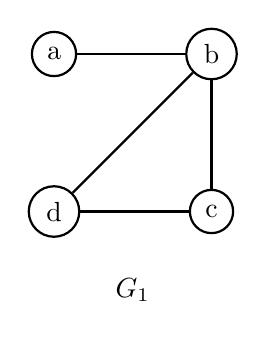
\begin{tikzpicture}
	\begin{scope}[every node/.style={circle,thick,draw}]
	\node (a) at (0,2) {a};
	\node (b) at (2,2) {b};
	\node (c) at (2,0) {c};
	\node (d) at (0,0) {d};
	\end{scope}
	\begin{scope}[every edge/.style={draw=black,thick}]
	\path (a) edge (b);
	\path (b) edge (c);
	\path (b) edge (d);
	\path (c) edge (d);
	\end{scope}
	\node () at (1,-1) {$G_1$};
	\end{tikzpicture}
	\hspace{1.5cm}
	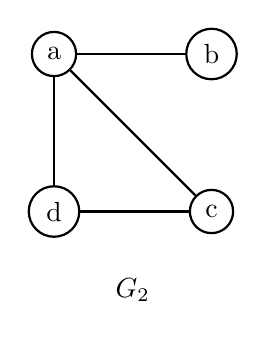
\begin{tikzpicture}
	\begin{scope}[every node/.style={circle,thick,draw}]
	\node (1) at (0,2) {a};
	\node (2) at (2,2) {b};
	\node (3) at (2,0) {c};
	\node (4) at (0,0) {d};
	\end{scope}
	\begin{scope}[every edge/.style={draw=black,thick}]
	\path (1) edge (2);
	\path (1) edge (3);
	\path (1) edge (4);
	\path (3) edge (4);
	\end{scope}
	\node () at (1,-1) {$G_2$};
	\end{tikzpicture}
	\caption{Nice pictures}
	\label{tikz:graphs}
\end{figure}


\begin{figure}
	\centering
	\begin{tikzpicture}[node distance=6cm]
	\node (a) [rect] {A Big Blue Block};
	\node (b) [oval, right of=a] {And His Oval Friend};
	\draw [line] (a) -- (b);
	\end{tikzpicture}
	\caption{Nice pictures}
	\label{tikz:graphs}
\end{figure}

\section{Development Approach}
An incremental development approach was used through out the construction of this application. The first task was to 
\section{Testing}
No test suites were used to test this application however there was considerable manual testing done with each iteration completed. Any bugs found were recorded and given a priority. The bugs were then fixed based on priority 
\section{Use of GitHub}
\section{Selection of Technologies to be used}




\chapter{Technology Review}
About seven to ten pages.
\begin{itemize}
\item Describe each of the technologies you used at a conceptual level. Standards, Database Model (e.g. MongoDB, CouchDB), XMl, WSDL, JSON, JAXP.
\item Use references (IEEE format, e.g. [1]), Books, Papers, URLs (timestamp) – sources should be authoritative. 
\end{itemize}

\section{XML}
Here's some nicely formatted XML:
\begin{minted}{xml}
<this>
  <looks lookswhat="good">
    Good
  </looks>
</this>
\end{minted}

\chapter{System Design}
As many pages as needed.
\begin{itemize}
\item Architecture, UML etc. An overview of the different components of the system. Diagrams etc… Screen shots etc.
\end{itemize}

\begin{table}[h]
  \centering
  \begin{tabular}{x{2cm}p{3cm}}
    \toprule \\
    Column 1 & Column 2 \\
    \midrule \\
    Rows 2.1 & Row 2.2 \\
    \bottomrule
  \end{tabular}
  \caption{A table.}
  \label{table:mytable}
\end{table}

\chapter{System Evaluation}
As many pages as needed.
\begin{itemize}
\item Prove that your software is robust. How? Testing etc. 
\item Use performance benchmarks (space and time) if algorithmic.
\item Measure the outcomes / outputs of your system / software against the objectives from the Introduction.
\item Highlight any limitations or opportuni-ties in your approach or technologies used.
\end{itemize}

\chapter{Conclusion}
About three pages.

\begin{itemize}
\item Briefly summarise your context and ob-jectives (a few lines).
\item Highlight your findings from the evalua-tion section / chapter and any opportuni-ties identified.
\end{itemize}

